\documentclass[11pt]{article}

% ---------- Packages ----------
\usepackage[a4paper,margin=1in]{geometry}
\usepackage{amsmath,amssymb,mathtools}
\usepackage{physics}       % for \dd, \partial, etc.
\usepackage{microtype}
\usepackage{enumitem}
\setlist{nosep}
\usepackage{tikz}
\usetikzlibrary{arrows.meta,calc,angles,quotes,decorations.pathreplacing}
\usepackage{pgfplots}
\pgfplotsset{compat=1.18}

% ---------- Macros ----------
\newcommand{\C}{\mathbb{C}}
\newcommand{\R}{\mathbb{R}}
\newcommand{\ii}{\mathrm{i}}
\newcommand{\dz}{\,\mathrm{d}z}
\newcommand{\dzbar}{\,\mathrm{d}\bar z}
\newcommand{\dx}{\,\mathrm{d}x}
\newcommand{\dy}{\,\mathrm{d}y}
\newcommand{\e}{\mathrm{e}}
\newcommand{\Ree}{\operatorname{Re}}
\newcommand{\Imm}{\operatorname{Im}}

\newtheorem{definition}{Definition}
\newtheorem{remark}{Remark}
\newtheorem{example}{Example}
\newtheorem{proposition}{Proposition}
\newtheorem{exercise}{Exercise}

% ---------- Title ----------
\title{\Large Visualizing and Formalizing {$\partial_z$}, {$dz$}, and Examples of Holomorphic vs.\ Non-Holomorphic Behavior}
\author{ }
\date{ }

\begin{document}
	\maketitle
	
	\section*{Aim}
	We give a formal derivation of the complex differential operators
	\[
	\partial_z := \tfrac12(\partial_x - \ii\,\partial_y),\qquad
	\partial_{\bar z} := \tfrac12(\partial_x + \ii\,\partial_y),
	\]
	explain their dual pairing with the complex $1$-forms
	\[
	dz = dx + \ii\,dy,\qquad d\bar z = dx - \ii\,dy,
	\]
	and provide \emph{concrete} examples (with computations) that sharply distinguish holomorphic from non-holomorphic functions. TikZ figures illustrate the geometry.
	
	\section{Coordinate change and the origin of the factor $\tfrac12$}
	Set
	\[
	z = x + \ii y,\qquad \bar z = x - \ii y.
	\]
	Then
	\[
	\begin{pmatrix} dz \\ d\bar z \end{pmatrix}
	=
	\underbrace{\begin{pmatrix} 1 & \ii \\ 1 & -\ii \end{pmatrix}}_{A}
	\begin{pmatrix} dx \\ dy \end{pmatrix}.
	\]
	Vector fields transform by the inverse transpose:
	\[
	\begin{pmatrix} \partial_x \\ \partial_y \end{pmatrix}
	= A^{-T} \begin{pmatrix} \partial_z \\ \partial_{\bar z} \end{pmatrix}.
	\]
	Since \(A^{-1}=\tfrac12\begin{pmatrix} 1 & 1 \\ -\ii & \ii\end{pmatrix}\), we have
	\[
	A^{-T}=\tfrac12\begin{pmatrix} 1 & -\ii \\ 1 & \ii\end{pmatrix},
	\quad\Rightarrow\quad
	\boxed{\;
		\partial_z=\tfrac12(\partial_x-\ii\partial_y),\quad
		\partial_{\bar z}=\tfrac12(\partial_x+\ii\partial_y)\;}.
	\]

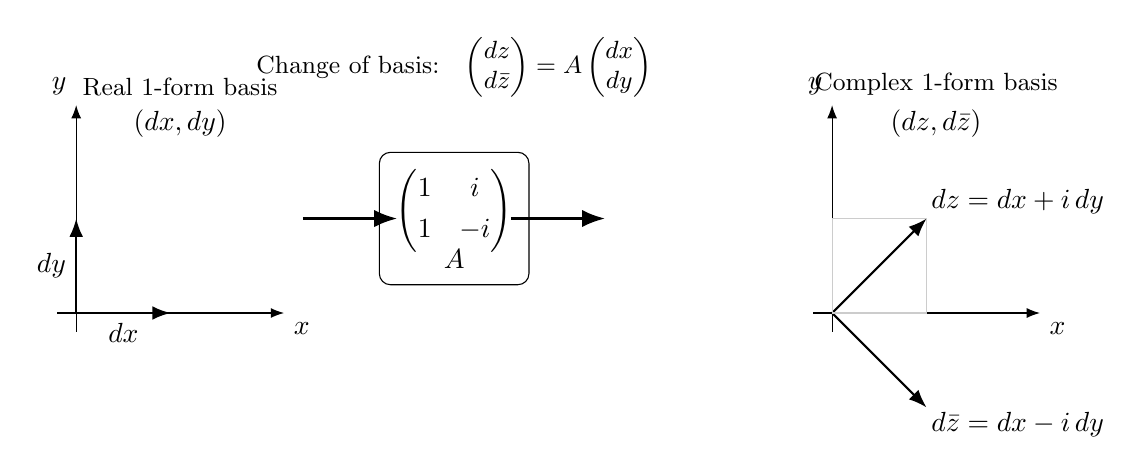
\begin{tikzpicture}[>=Latex, scale=1.2]
	
	% ----- LEFT: real basis (dx, dy)
	\begin{scope}
		% axes
		\draw[->] (-0.2,0) -- (2.2,0) node[below right] {$x$};
		\draw[->] (0,-0.2) -- (0,2.2) node[above left] {$y$};
		
		% basis vectors
		\draw[->,thick] (0,0) -- (1,0) node[midway,below] {$dx$};
		\draw[->,thick] (0,0) -- (0,1) node[midway,left] {$dy$};
		
		% title
		\node[above] at (1.1,2.2) {\small Real 1-form basis};
		\node at (1.1,2.0) {\(\ (dx,dy)\ \)};
	\end{scope}
	
	% ----- MIDDLE: the matrix A as a label
	\node[draw, rounded corners, inner xsep=6pt, inner ysep=6pt, align=center] (A) at (4,1) 
	{$\displaystyle 
		\begin{pmatrix} 1 & i \\[3pt] 1 & -i \end{pmatrix}$\\[-2pt]
		\(\,A\,\)};
	
	% arrows indicating “mapping”
	\draw[->,very thick] (2.4,1) -- (3.4,1);
	\draw[->,very thick] (4.6,1) -- (5.6,1);
	
	% ----- RIGHT: complex basis (dz, d\bar z)
	\begin{scope}[xshift=8cm]
		% axes (same background axes for reference)
		\draw[->] (-0.2,0) -- (2.2,0) node[below right] {$x$};
		\draw[->] (0,-0.2) -- (0,2.2) node[above left] {$y$};
		
		% diagonals representing dz and d\bar z directions (real geometry picture)
		\draw[->,thick] (0,0) -- (1,1) node[above right=-2pt] {$dz=dx+i\,dy$};
		\draw[->,thick] (0,0) -- (1,-1) node[below right=-2pt] {$d\bar z=dx-i\,dy$};
		
		% light guide: unit square
		\draw[gray!40] (0,0) rectangle (1,1);
		
		% title
		\node[above] at (1.1,2.2) {\small Complex 1-form basis};
		\node at (1.1,2.0) {\(\ (dz,d\bar z)\ \)};
	\end{scope}
	
	% legend for what the figure means
	\node[align=center] at (4,2.6)
	{\small Change of basis:\quad
		$\begin{pmatrix}dz\\ d\bar z\end{pmatrix}
		= A \begin{pmatrix}dx\\ dy\end{pmatrix}$};
	
\end{tikzpicture}


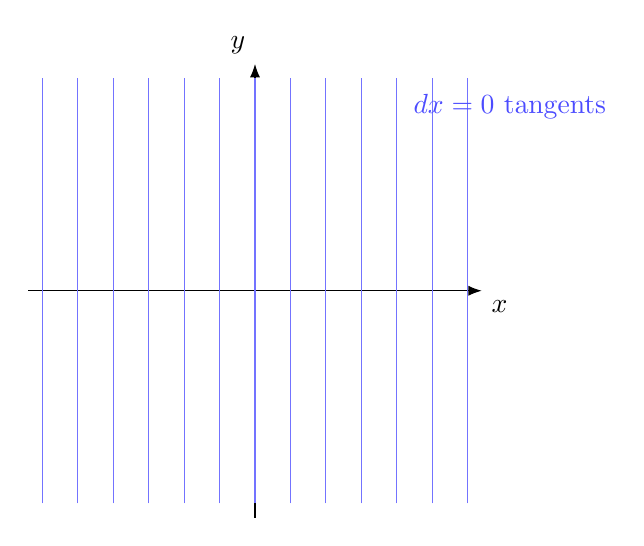
\begin{tikzpicture}[scale=0.9,>=Latex]
% Axes
\draw[->] (-3.2,0) -- (3.2,0) node[below right] {$x$};
\draw[->] (0,-3.2) -- (0,3.2) node[above left] {$y$};

% === Foliations as level sets ===
% dx = d(x): vertical lines x = const
\foreach \x in {-3,-2.5,...,3}
\draw[blue!55] (\x,-3) -- (\x,3);
\node[blue!70,anchor=west] at (2.1,2.6) {$dx=0$ tangents};
\end{tikzpicture}

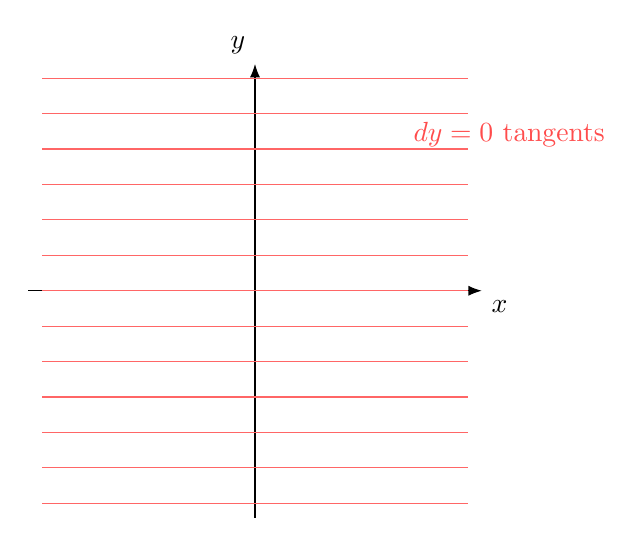
\begin{tikzpicture}[scale=0.9,>=Latex]
% Axes
\draw[->] (-3.2,0) -- (3.2,0) node[below right] {$x$};
\draw[->] (0,-3.2) -- (0,3.2) node[above left] {$y$};

%% === Foliations as level sets ===
%% dx = d(x): vertical lines x = const
%\foreach \x in {-3,-2.5,...,3}
%\draw[blue!55] (\x,-3) -- (\x,3);
%\node[blue!70,anchor=west] at (2.1,2.6) {$dx=0$ tangents};

% dy = d(y): horizontal lines y = const
\foreach \y in {-3,-2.5,...,3}
\draw[red!60] (-3,\y) -- (3,\y);
\node[red!70,anchor=west] at (2.1,2.2) {$dy=0$ tangents};
	
%	% dx+dy = d(x+y): lines x+y = const  (slope -1)
%	\foreach \c in {-6,-5.5,...,6}
%	\draw[green!60] (-3,\c+3) -- (3,\c-3);
%	\node[green!70,anchor=west] at (2.1,1.8) {$dx+dy=0$ tangents};
%	
%	% dx-dy = d(x-y): lines x-y = const  (slope +1)
%	\foreach \c in {-6,-5.5,...,6}
%	\draw[violet!60] (-3,-\c-3) -- (3,-\c+3);
%	\node[violet!70,anchor=west] at (2.1,1.4) {$dx-dy=0$ tangents};
%	
%	% Legend box connecting to dz
%	\node[align=left, draw, rounded corners, fill=white, opacity=0.95, text opacity=1, below right] at (-3.05,3.05) {%
	%		\(\begin{aligned}
		%			dz &= dx + i\,dy\\
		%			\Re(dz) &= dx \;\Rightarrow\; x=\text{const}\\
		%			\Im(dz) &= dy \;\Rightarrow\; y=\text{const}
		%		\end{aligned}\)
	%	};
%	
%	% Small arrows showing kernel directions for each real form
%	\draw[->,blue!80,thick] (0,0) -- (0,1) node[midway,left] {\(\ker dx\)};
%	\draw[->,red!80,thick]  (0,0) -- (1,0) node[midway,below] {\(\ker dy\)};
%	\draw[->,green!80,thick] (0,0) -- (1,-1) node[near end,below right=-1pt] {\(\ker(dx{+}dy)\)};
%	\draw[->,violet!80,thick] (0,0) -- (1,1) node[near end,above right=-1pt] {\(\ker(dx{-}dy)\)};
\end{tikzpicture}

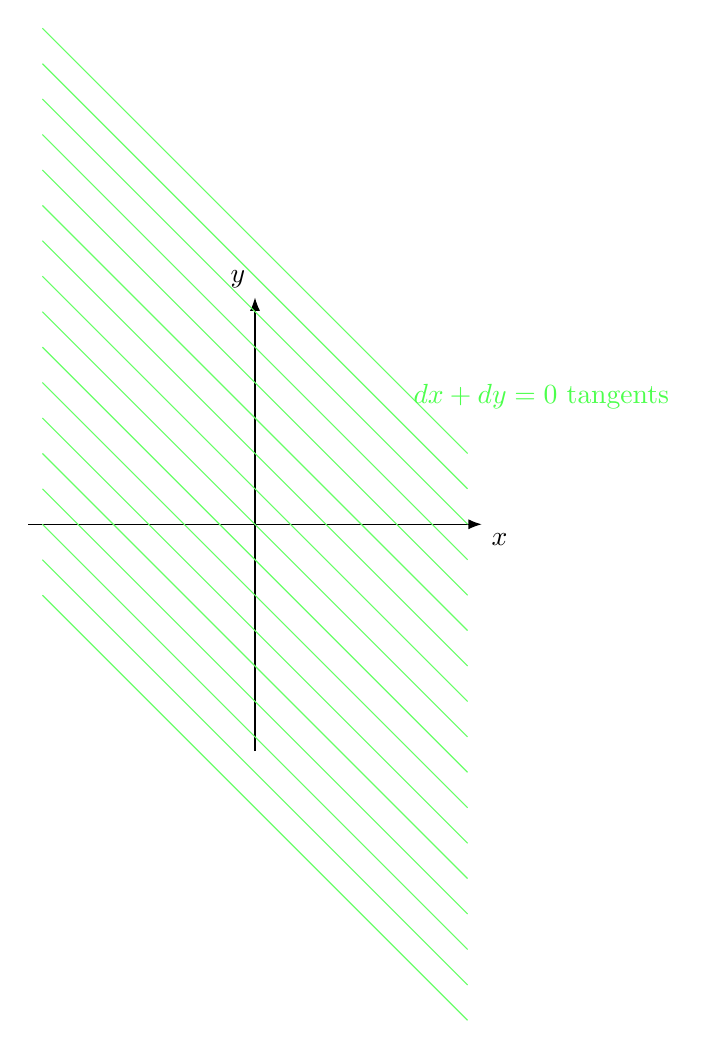
\begin{tikzpicture}[scale=0.9,>=Latex]
% Axes
\draw[->] (-3.2,0) -- (3.2,0) node[below right] {$x$};
\draw[->] (0,-3.2) -- (0,3.2) node[above left] {$y$};

% dx+dy = d(x+y): lines x+y = const  (slope -1)
\foreach \c in {-4,-3.5,...,4}
\draw[green!60] (-3,\c+3) -- (3,\c-3);
\node[green!70,anchor=west] at (2.1,1.8) {$dx+dy=0$ tangents};	
\end{tikzpicture}

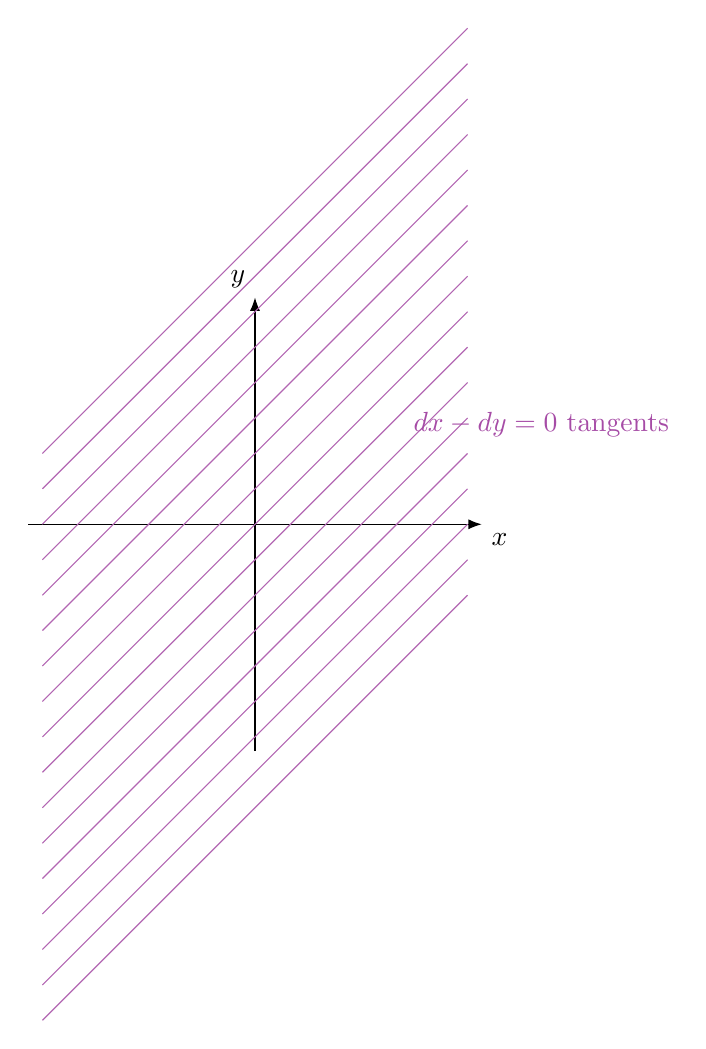
\begin{tikzpicture}[scale=0.9,>=Latex]
% Axes
\draw[->] (-3.2,0) -- (3.2,0) node[below right] {$x$};
\draw[->] (0,-3.2) -- (0,3.2) node[above left] {$y$};

% dx-dy = d(x-y): lines x-y = const  (slope +1)
\foreach \c in {-4,-3.5,...,4}
\draw[violet!60] (-3,-\c-3) -- (3,-\c+3);
\node[violet!70,anchor=west] at (2.1,1.4) {$dx-dy=0$ tangents};
	
%	% Legend box connecting to dz
%	\node[align=left, draw, rounded corners, fill=white, opacity=0.95, text opacity=1, below right] at (-3.05,3.05) {%
	%		\(\begin{aligned}
		%			dz &= dx + i\,dy\\
		%			\Re(dz) &= dx \;\Rightarrow\; x=\text{const}\\
		%			\Im(dz) &= dy \;\Rightarrow\; y=\text{const}
		%		\end{aligned}\)
	%	};
%	
%	% Small arrows showing kernel directions for each real form
%	\draw[->,blue!80,thick] (0,0) -- (0,1) node[midway,left] {\(\ker dx\)};
%	\draw[->,red!80,thick]  (0,0) -- (1,0) node[midway,below] {\(\ker dy\)};
%	\draw[->,green!80,thick] (0,0) -- (1,-1) node[near end,below right=-1pt] {\(\ker(dx{+}dy)\)};
%	\draw[->,violet!80,thick] (0,0) -- (1,1) node[near end,above right=-1pt] {\(\ker(dx{-}dy)\)};
\end{tikzpicture}

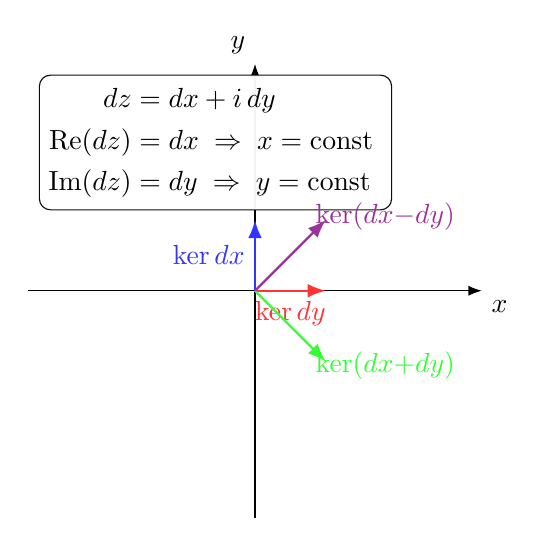
\begin{tikzpicture}[scale=0.9,>=Latex]
% Axes
\draw[->] (-3.2,0) -- (3.2,0) node[below right] {$x$};
\draw[->] (0,-3.2) -- (0,3.2) node[above left] {$y$};

% Legend box connecting to dz
\node[align=left, draw, rounded corners, fill=white, opacity=0.95, text opacity=1, below right] at (-3.05,3.05) {%
		\(\begin{aligned}
				dz &= dx + i\,dy\\
				\Re(dz) &= dx \;\Rightarrow\; x=\text{const}\\
				\Im(dz) &= dy \;\Rightarrow\; y=\text{const}
			\end{aligned}\)
};

% Small arrows showing kernel directions for each real form
\draw[->,blue!80,thick] (0,0) -- (0,1) node[midway,left] {\(\ker dx\)};
\draw[->,red!80,thick]  (0,0) -- (1,0) node[midway,below] {\(\ker dy\)};
\draw[->,green!80,thick] (0,0) -- (1,-1) node[near end,below right=-1pt] {\(\ker(dx{+}dy)\)};
\draw[->,violet!80,thick] (0,0) -- (1,1) node[near end,above right=-1pt] {\(\ker(dx{-}dy)\)};
\end{tikzpicture}

	\newpage
	\section{Dual pairing and holomorphicity}
	By construction,
	\[
	dz(\partial_z)=1,\quad dz(\partial_{\bar z})=0,\qquad
	d\bar z(\partial_{\bar z})=1,\quad d\bar z(\partial_z)=0.
	\]
	For a \(C^1\) function \(f\colon\C\to\C\),
	\[
	df = f_x\,dx + f_y\,dy = f_z\,dz + f_{\bar z}\,d\bar z,
	\quad\text{where}\quad
	f_z=\tfrac12(f_x-\ii f_y),\ \ f_{\bar z}=\tfrac12(f_x+\ii f_y).
	\]
	\emph{Holomorphic} means \(f_{\bar z}=0\), equivalently \(df=f_z\,dz\) (no \(d\bar z\)-part).
	
	\section{Geometric action of $dz$}
	For a real tangent vector \(v=a\,\partial_x+b\,\partial_y\),
	\[
	dz(v)=a+\ii b.
	\]
	Thus \(dz\) converts a real direction into a complex number whose modulus is speed and whose argument is direction.
	
	\begin{center}
		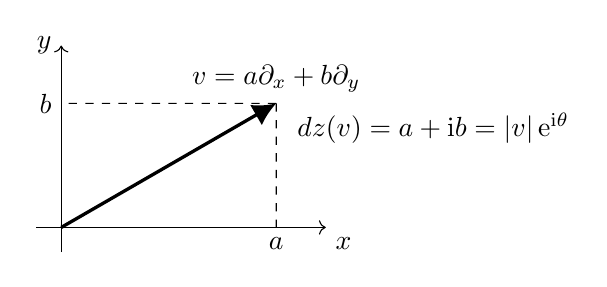
\begin{tikzpicture}[scale=1.05]
			% axes
			\draw[->] (-0.3,0) -- (3.2,0) node[below right] {$x$};
			\draw[->] (0,-0.3) -- (0,2.2) node[left] {$y$};
			% vector v
			\coordinate (O) at (0,0);
			\coordinate (V) at (2.6,1.5);
			\draw[very thick, -{Latex[width=3mm]}] (O) -- (V) node[above] {$v=a\partial_x+b\partial_y$};
			% projections
			\draw[dashed] (V) -- (2.6,0) node[below] {$a$};
			\draw[dashed] (V) -- (0,1.5) node[left] {$b$};
			% angle
%			\pic[draw, ->, angle eccentricity=1.35, angle radius=1cm] {angle = (1,0)--(0,0)--(2.6,1.5)};
			\node at (4.5,1.2) {$dz(v)=a+\ii b=|v|\,\e^{\ii\theta}$};
		\end{tikzpicture}
		\smallskip
		\small Fig.~1. The $1$-form \(dz\) encodes magnitude/direction as a complex number.
	\end{center}
	
	\section{Penetrating examples}
	We now compute \(f_z, f_{\bar z}\) and \(df\) explicitly and interpret the results geometrically.
	
	\subsection*{Example A (holomorphic): \boldmath\(f(z)=z^2\)}
	Write \(f(x,y)=(x+\ii y)^2=x^2-y^2+2\ii xy\). Then
	\[
	f_x=2x+2\ii y,\qquad f_y=-2y+2\ii x.
	\]
	Hence
	\[
	f_z=\tfrac12(f_x-\ii f_y)=\tfrac12\bigl[(2x+2\ii y)-\ii(-2y+2\ii x)\bigr]=2(x+\ii y)=2z,
	\]
	\[
	f_{\bar z}=\tfrac12(f_x+\ii f_y)=\tfrac12\bigl[(2x+2\ii y)+\ii(-2y+2\ii x)\bigr]=0.
	\]
	Thus \(df=2z\,dz\) and \(f\) is holomorphic. Along any vector \(v\),
	\[
	df(v)=2z\cdot dz(v)=2z\,(a+\ii b).
	\]
	\emph{Geometric meaning:} the complex directional derivative is the complex number \(2z\) times the complex encoding of \(v\).
	
	\subsection*{Example B (non-holomorphic): \boldmath\(f(z)=|z|^2=z\bar z=x^2+y^2\)}
	Here
	\[
	f_x=2x,\qquad f_y=2y,\quad
	f_z=\tfrac12(2x-\ii\cdot 2y)=x-\ii y=\bar z,\quad
	f_{\bar z}=\tfrac12(2x+\ii\cdot 2y)=x+\ii y=z.
	\]
	So
	\[
	df=\bar z\,dz+z\,d\bar z,
	\]
	and \(f_{\bar z}=z\neq 0\) unless \(z=0\): \emph{not holomorphic}. Note that the gradient in real terms points radially; the presence of a \(d\bar z\)-piece records the anti-holomorphic contribution.
	
	\begin{center}
		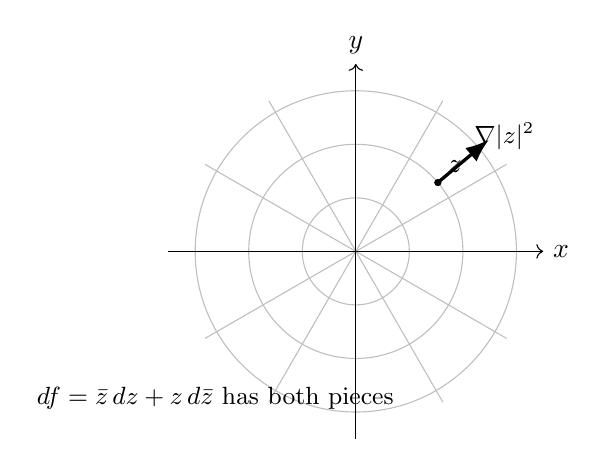
\begin{tikzpicture}[scale=0.85]
			% grid
			\foreach \r in {0.8,1.6,2.4} \draw[lightgray] (0,0) circle (\r);
			\foreach \ang in {0,30,...,330} \draw[lightgray] (0,0) -- (\ang:2.6);
			\draw[->] (-2.8,0) -- (2.8,0) node[right] {$x$};
			\draw[->] (0,-2.8) -- (0,2.8) node[above] {$y$};
			% sample point and gradient
			\draw[fill] (40:1.6) circle (1.3pt) node[above right] {$z$};
			\draw[very thick, -{Latex[length=3mm]}] (40:1.6) -- ++(40:1.0) node[midway, above right] {\small $\nabla |z|^2$};
			\node at (-2.1,-2.2) {\small $df=\bar z\,dz+z\,d\bar z$ has both pieces};
		\end{tikzpicture}
		
		\smallskip
		\small Fig.~2. For \(f=|z|^2\), level sets are circles; $df$ has a \(d\bar z\)-part, so \(f\) is not holomorphic.
	\end{center}
	
	\subsection*{Example C (anti-holomorphic): \boldmath\(f(z)=\bar z\)}
	We have \(f_x=1,\ f_y=-\ii\), so
	\[
	f_z=\tfrac12(1-\ii\cdot(-\ii))=0,\qquad f_{\bar z}=\tfrac12(1+\ii\cdot(-\ii))=1,
	\]
	hence \(df=d\bar z\). This is \emph{purely} anti-holomorphic: \(dz\) is annihilated and only $d\bar z$ survives.
	
	\subsection*{Example D (logarithmic/winding): \boldmath\( \omega=\dfrac{dz}{z}\) on \(\C^\times\)}
	Write \(z=re^{\ii\theta}\) with \(r>0\). Then
	\[
	\frac{dz}{z}=\frac{d(re^{\ii\theta})}{re^{\ii\theta}}=\frac{dr}{r}+\ii\,d\theta
	= d(\log r)+\ii\,d\arg z.
	\]
	\(\Ree(\omega)\) measures radial change, \(\Imm(\omega)\) measures angular change. For the circle \(\gamma(t)=R\,e^{\ii t}\), \(t\in[0,2\pi]\),
	\[
	\oint_\gamma \frac{dz}{z}=\ii\int_0^{2\pi} dt=2\pi\ii.
	\]
	
	\begin{center}
		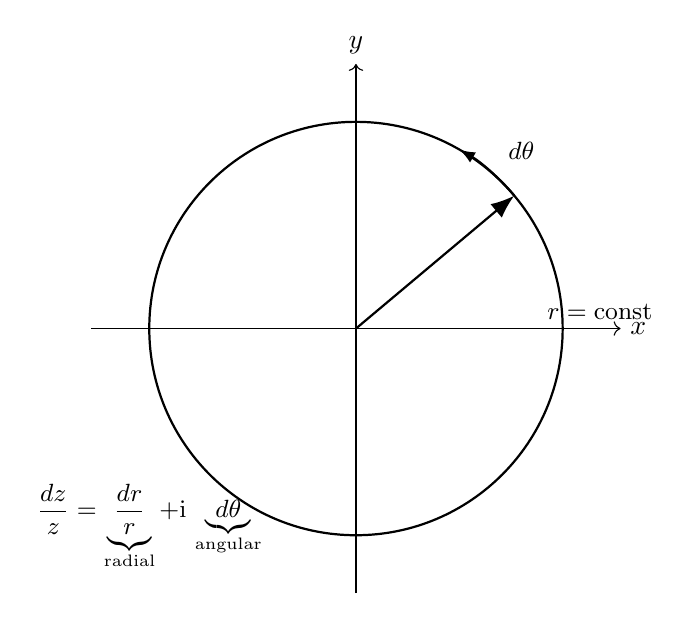
\begin{tikzpicture}[scale=1.05]
			\draw[->] (-3.2,0) -- (3.2,0) node[right] {$x$};
			\draw[->] (0,-3.2) -- (0,3.2) node[above] {$y$};
			\draw[thick] (0,0) circle (2.5);
			\node at (2.95,0.2) {\small $r=\text{const}$};
			\draw[thick, -{Latex[length=3mm]}] (0,0) -- (40:2.5);
%			\pic[draw, ->, "$\theta$", angle eccentricity=1.35, angle radius=1cm] {angle = (1,0)--(0,0)--(40:1)};
			\draw[thick, -{Latex[length=2mm]}] (40:2.5) arc (40:60:2.5);
			\node at (2.0,2.15) {\small $d\theta$};
			\node at (-2.5,-2.4) {\small $\displaystyle \frac{dz}{z}=\underbrace{\frac{dr}{r}}_{\text{radial}}+\ii\,\underbrace{d\theta}_{\text{angular}}$};
		\end{tikzpicture}
		
		\smallskip
		\small Fig.~3. The decomposition of \(\frac{dz}{z}\) as radial + angular.
	\end{center}
	
	\section{Why $\partial_z$ and $\partial_{\bar z}$ matter}
	Given a $C^1$ function \(f\),
	\[
	\partial_z f = f_z,\qquad \partial_{\bar z} f = f_{\bar z}.
	\]
	Holomorphicity is the single linear condition \(\partial_{\bar z} f=0\), equivalently, \(df\) has \emph{no} $d\bar z$ component. This compresses the Cauchy--Riemann equations into a basis statement: ``\(df\) is complex-linear.''
	
	\section{Operational ``recipe'' (ready to use)}
	Let \(f(x,y)\) be given.
	\[
	\boxed{
		\begin{aligned}
			&f_z=\tfrac12\left(\frac{\partial f}{\partial x}-\ii\frac{\partial f}{\partial y}\right),\qquad
			f_{\bar z}=\tfrac12\left(\frac{\partial f}{\partial x}+\ii\frac{\partial f}{\partial y}\right),\\
			&df=f_z\,dz+f_{\bar z}\,d\bar z,\quad
			\text{$f$ holomorphic } \Longleftrightarrow f_{\bar z}\equiv 0.
	\end{aligned}}
	\]
	
	\section{A visual of the complex coframe}
	Although \(\partial_z,\partial_{\bar z}\) are complex combinations of real directions, the \emph{pairing} with $dz,d\bar z$ is exact: one kills the other.
	
	\begin{center}
		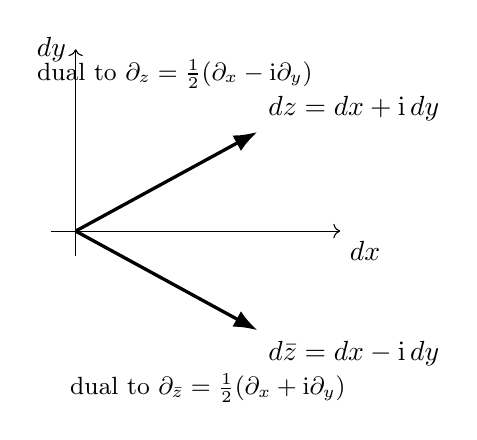
\begin{tikzpicture}[scale=1.05]
			\draw[->] (-0.3,0) -- (3.2,0) node[below right] {$dx$};
			\draw[->] (0,-0.3) -- (0,2.2) node[left] {$dy$};
			% dz and d\bar z vectors (as co-vectors illustrated by arrows for intuition)
			\draw[very thick, -{Latex[length=3mm]}] (0,0) -- (2.2,1.2) node[above right] {$dz=dx+\ii\,dy$};
			\draw[very thick, -{Latex[length=3mm]}] (0,0) -- (2.2,-1.2) node[below right] {$d\bar z=dx-\ii\,dy$};
			\node at (1.2,1.9) {\small dual to $\partial_z=\tfrac12(\partial_x-\ii\partial_y)$};
			\node at (1.6,-1.9) {\small dual to $\partial_{\bar z}=\tfrac12(\partial_x+\ii\partial_y)$};
		\end{tikzpicture}
		
		\smallskip
		\small Fig.~4. Heuristic picture: $dz$ detects $\partial_z$ and kills $\partial_{\bar z}$; $d\bar z$ does the opposite.
	\end{center}
	
	\section*{Appendix: fully worked micro-examples}
	\begin{example}[Directional values of $dz$]
		Along $\partial_x$, $dz(\partial_x)=1$; along $\partial_y$, $dz(\partial_y)=\ii$; along $\partial_x+\partial_y$, $dz=1+\ii$.
	\end{example}
	
	\begin{example}[$f(z)=\e^z$ is holomorphic]
		$f_x=\e^x\cos y + \ii\,\e^x\sin y,\; f_y=-\e^x\sin y + \ii\,\e^x\cos y$ so
		\(
		f_z=\tfrac12(f_x-\ii f_y)=\e^{x+\ii y}=\e^z,\;
		f_{\bar z}=0,
		\)
		and \(df=\e^z\,dz\).
	\end{example}
	
	\begin{example}[$f(z)=\overline{z}^2$ is anti-holomorphic]
		$f_x=2x,\ f_y=-2\ii y$ so \(f_z=0,\ f_{\bar z}=2\bar z\), hence \(df=2\bar z\,d\bar z\).
	\end{example}
	
	\section*{Exercises (with short answers)}
	\begin{enumerate}[label=\arabic*)]
		\item Show directly from definitions that \(dz(\partial_{\bar z})=0\) and \(d\bar z(\partial_z)=0\).
		\item For \(f(z)=x^3-3xy^2 + \ii(3x^2 y - y^3)\), compute \(f_z,f_{\bar z}\) and determine holomorphicity. (Ans: \(f_{\bar z}=0\): this is the cubic $z^3$.)
		\item Let $\gamma(t)=R\e^{\ii t}$, $t\in[0,2\pi]$. Compute $\oint_\gamma dz$ and $\oint_\gamma dz/z$. (Ans: $0$ and $2\pi\ii$.)
	\end{enumerate}
	
\end{document}
